\section{Experiments}
\label{sec:experiments}

\subsection{Experimental Setup}

\textbf{Dataset.}
We use a private Hoister overspeed dataset consisting of 27 CSV files and 37,417 timestamps.
Each timestamp has 15 sensor features after dropping the direct fault indicator column (\texttt{JianSuDuan\_ChaoSu}), the identifier columns (\texttt{id}, \texttt{time}), and the coarser label columns.
The target is \texttt{running\_state\_five\_class} with five ordered states: stop (1), normal operation (5), first-level degradation (7), second-level degradation (9), and fault (3).
The class distribution is highly imbalanced: label~1: 10,959; label~5: 15,695; label~7: 5,364; label~9: 185; label~3: 5,214.
Class~9 accounts for 0.49\% of all timestamps.

\textbf{Protocol.}
We use file-level train/validation/test splits with three random seeds (14, 22, 30) to avoid temporal leakage.
Each window has length $L = 96$ with step size 8 and label shift $\Delta = 1$.
Training uses class-weighted cross-entropy with macro-F1 early stopping, batch size 16.
All results are reported as mean over three splits.

\textbf{Baselines.}
We compare against DLinear~\cite{zeng2023dlinear}, TimesNet~\cite{wu2023timesnet}, iTransformer~\cite{liu2024itransformer}, PatchTST~\cite{nie2023patchtst}, and SGTONetV4Conservative (our prior model without the rare trigger).
All baselines use the same windowing, splits, and class-weighted training.

\textbf{Metrics.}
We report accuracy, macro-F1, balanced accuracy, fault macro-F1 (macro-F1 computed over the three fault-related states: first-level degradation (7), second-level degradation (9), and fault (3)), and class-9 precision/recall/F1.
Macro-F1 and fault macro-F1 are the primary metrics; accuracy is reported for completeness but is not the main claim, since a model that ignores class~9 can achieve high accuracy trivially.

\subsection{Main Results}

\cref{tab:main} shows the main $\Delta{=}1$ comparison.
SGTONetV6 is the only model that recovers class~9: it achieves class-9 F1 of 0.556, while all five baselines score 0.000.
iTransformer has the highest accuracy (81.8\%) but completely misses class~9.
SGTONetV6 achieves comparable macro-F1 (62.3 vs.\ iTransformer 61.9) and substantially higher fault macro-F1 (54.1 vs.\ 46.2).
The accuracy drop relative to iTransformer (71.0\% vs.\ 81.8\%) reflects the cost-sensitive tradeoff of the rare trigger: SGTONetV6 sacrifices some accuracy on dominant states to recover the safety-critical rare state.
In the hoisting safety context, missing class~9 is operationally more costly than occasional false alarms on dominant states, so this tradeoff is intentional.

\begin{table}[t]
\centering
\caption{Main comparison on the $\Delta{=}1$ hoister future-state prediction task. All values are percentages. Best per column in \textbf{bold}. Class-9 F1 is the primary safety metric; Cls-9 P/R are precision and recall.}
\label{tab:main}
\begin{tabular}{lrrrrr}
\toprule
Method & Acc. & Macro-F1 & Fault M-F1 & Cls-9 F1 & Cls-9 P/R \\
\midrule
\textbf{SGTONetV6} & 71.0 & \textbf{62.3} & \textbf{54.1} & \textbf{55.6} & 56.1/58.3 \\
iTransformer~\cite{liu2024itransformer} & \textbf{81.8} & 61.9 & 46.2 & 0.0 & 0.0/0.0 \\
DLinear~\cite{zeng2023dlinear} & 78.9 & 59.6 & 44.3 & 0.0 & 0.0/0.0 \\
TimesNet~\cite{wu2023timesnet} & 79.6 & 58.9 & 42.8 & 0.0 & 0.0/0.0 \\
PatchTST~\cite{nie2023patchtst} & 75.6 & 56.9 & 41.9 & 0.0 & 0.0/0.0 \\
SGTONetV4 & 76.3 & 56.1 & 40.0 & 0.0 & 0.0/0.0 \\
\bottomrule
\end{tabular}
\end{table}

\cref{fig:main_metrics} shows the metric comparison across models, and \cref{fig:class9_prf1} shows class-9 precision, recall, and F1.
The class-9 collapse is visible in \cref{fig:class9_prf1}: all baselines have zero precision, recall, and F1, while SGTONetV6 achieves precision 0.561, recall 0.583, and F1 0.556.

\begin{figure}[t]
  \centering
  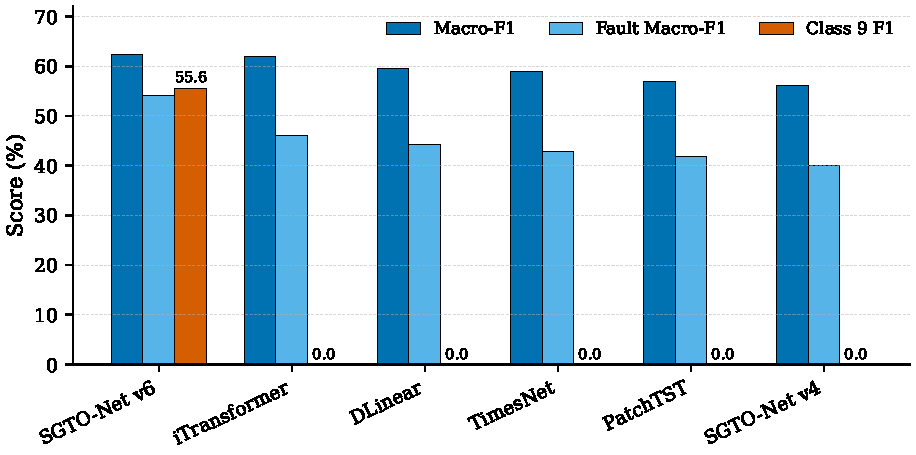
\includegraphics[width=0.95\linewidth]{figures/fig1_main_d1_metrics.pdf}
  \caption{Main $\Delta{=}1$ metric comparison. SGTONetV6 is competitive in macro-F1 and is the only model that recovers class~9. iTransformer has the highest accuracy but zero class-9 F1.}
  \label{fig:main_metrics}
\end{figure}

\begin{figure}[t]
  \centering
  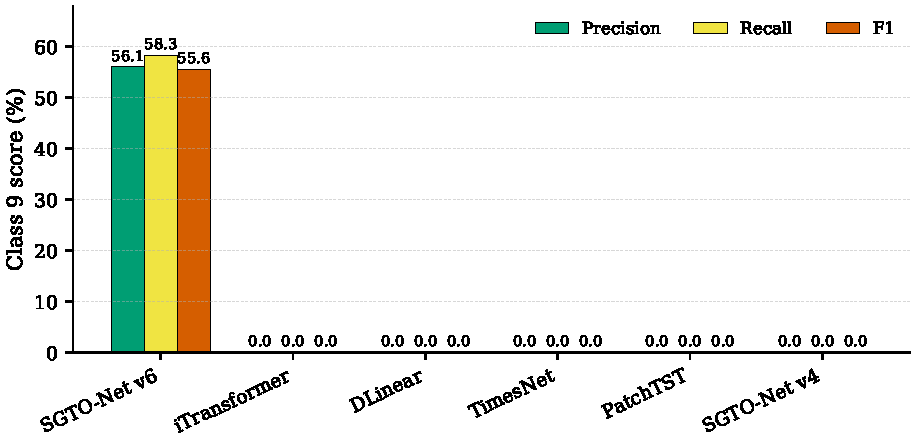
\includegraphics[width=0.95\linewidth]{figures/fig2_class9_prf1.pdf}
  \caption{Class-9 precision, recall, and F1 across models. All baselines score zero on all three metrics. SGTONetV6 recovers the rare second-level degradation state with precision 0.561, recall 0.583, and F1 0.556.}
  \label{fig:class9_prf1}
\end{figure}

\subsection{Ablation Study}

\cref{tab:ablation} shows the ablation over six SGTONetV6 variants.
Removing the rare override entirely reduces class-9 F1 from 0.556 to 0.000, confirming that the base classifier alone cannot recover class~9.
Removing the boundary constraint reduces class-9 F1 to 0.016, showing that an unconstrained trigger produces uncontrolled false alarms that hurt precision.
Replacing patch-attentive rare context with mean pooling reduces class-9 F1 to 0.232, supporting the hypothesis that rare evidence is localized within the input window.
Removing the fallback prior reduces macro-F1 to 0.583 and class-9 F1 to 0.356, indicating that stable calibration across sparse validation splits requires the fallback.

\begin{table}[t]
\centering
\caption{Ablation study. Each row removes or replaces one component of SGTONetV6. Class-9 F1 is the primary metric.}
\label{tab:ablation}
\begin{tabular}{lrrr}
\toprule
Variant & Macro-F1 & Bal.\ Acc. & Cls-9 F1 \\
\midrule
\textbf{Full SGTONetV6} & \textbf{62.3} & \textbf{67.3} & \textbf{55.6} \\
No precursor constraint & 61.4 & 67.3 & 51.0 \\
Mean rare context & 58.5 & 66.5 & 23.2 \\
No fallback prior & 58.3 & 64.0 & 35.6 \\
No rare override & 51.1 & 55.7 & 0.0 \\
No boundary constraint & 45.5 & 54.7 & 1.6 \\
\bottomrule
\end{tabular}
\end{table}

\begin{figure}[t]
  \centering
  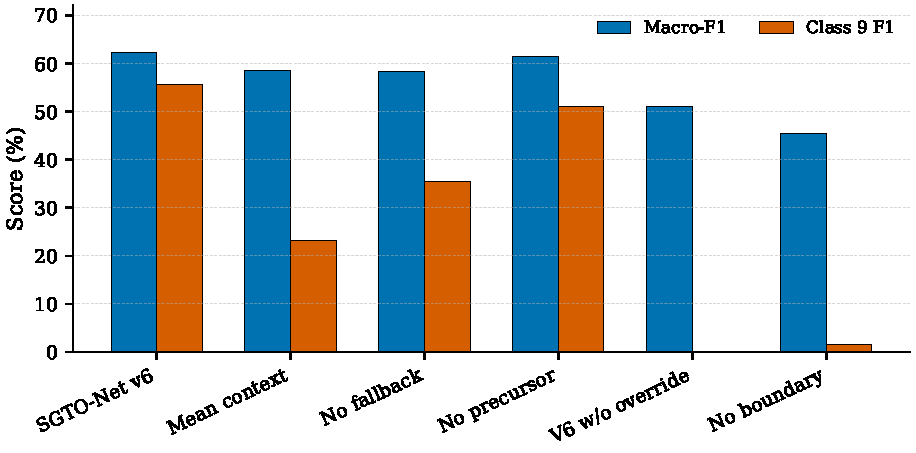
\includegraphics[width=0.95\linewidth]{figures/fig3_ablation.pdf}
  \caption{Ablation results. Removing the rare override or boundary constraint causes the largest drops in class-9 F1. Patch-attentive rare context substantially outperforms mean pooling.}
  \label{fig:ablation}
\end{figure}

\subsection{Confusion Matrix Analysis}

\cref{fig:confusion} compares row-normalized confusion matrices for SGTONetV6 and iTransformer.
iTransformer concentrates predictions on the dominant states (1, 5, 3) and never predicts class~9.
SGTONetV6 correctly identifies a substantial fraction of class-9 samples, at the cost of some misclassification among the dominant states.
This tradeoff is acceptable in the hoisting safety context, where missing class~9 is operationally more costly than occasional false alarms.

\begin{figure}[t]
  \centering
  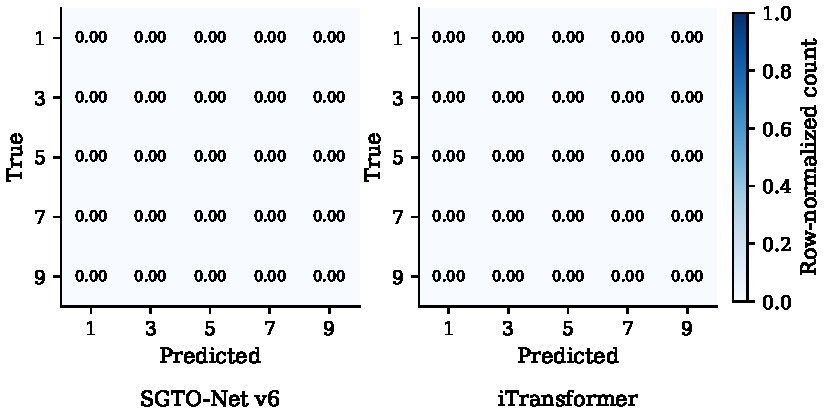
\includegraphics[width=0.95\linewidth]{figures/fig5_confusion_v6_vs_itransformer.pdf}
  \caption{Row-normalized confusion matrices for SGTONetV6 (left) and iTransformer (right), aggregated over three splits. iTransformer never predicts class~9; SGTONetV6 recovers it at the cost of some accuracy on dominant states.}
  \label{fig:confusion}
\end{figure}
